\documentclass[thesis]{subfiles}

\begin{document}

\OnlyInSubfile{\setcounter{chapter}{5}}

\chapter{Implementation of molecular simulation software}

\vskip\baselineskip

During my PhD, I also worked to implement molecular simulation software as part
of the Domino project. In this chapter I will this project and my contributions
to it, as well as some advanced simulation techniques I worked to incorporate in
Domino.

The first of these advanced methods is the Hybrid Monte Carlo simulation
technique, which join molecular dynamics and Monte Carlo in an attempt to get
the advantages of both. I will present the original method and some of the most
recent developments and improvements to it.

The second of these methods concern the treatment of electrostatic interactions
in the context of periodic boundary conditions. I will first describe the Ewald
summation technique, and some tricks for optimizing its implementation. Then I
will discuss the Wolf summation method as one alternative to Ewald summation
that only relies on a sum of pair terms.

\newpage
\section{Domino: extensible molecular simulations library}

Domino is a \cxx library that allow to run classical molecular simulations. In
this section I will present the code and my contributions to it, as well as some
of the goals and software architecture choices made to reach these goals.

Domino is written in \cxx, a computer programming language created in 1983 by
Bjarne Stroustrup as an extension of the C language. \cxx mainly adds
object-orientatation, functions overloading and generic programming to C. We
choose \cxx because it is a general purpose language, which we can use to
implement complex algorithms while retaining the ability to manage memory
allocations and the memory layout of data. These two last points are what allow
\cxx to run faster than \emph{managed} languages, where the users don't have
control over memory allocation, locality and layout.  Software written in \cxx
will not be inherently faster than say Python, but developers are able to
optimize it further. Domino uses the \cxx11 version of \cxx standard, which
brought major changes to \cxx, creating a subset of the language which is easier
to use correctly and more expressive.

In this section, I will assume some basic programming, \cxx and object-oriented
knowledge from the readers. There are a lot of great online resources on all of
these subjects, as well as books such as \emph{"\cxx Primer"} by Stanley B.
Lippman, Josée Lajoie, and Barbara E. Moo; or \emph{"Effective Modern \cxx"} by
Scott Meyers.

\subsection{Goals and architecture}

The main goal of Domino is to be an extensible classical molecular simulation
library. A software library is a collection of functions and classes working
together to provide some functionality. Domino provides facilities to run
classical Monte Carlo, molecular dynamics and energy minimization simulations.
We also tried to make it easy to use, and easy to extend, meaning it can be used
as a basis for the development of new molecular simulations methods.

These goals translate into some of the architectural choices: in particular, the
code needs to be simple to understand before being simple to extend. This means
I restricted myself to a simple subset of \cxx, not using complex template-based
meta-programming or deep class hierarchies.

Extensions points exist in two places in Domino. Classes that provide central
behavior, such as potentials or molecular dynamics integrators are manipulated
through pointers to a pure virtual base class --- or \emph{interface} ---
throughout the code. By creating a new class inheriting from this interface, it
is possible to add behavior to Domino without having to modify any of its
internal source code. For example, the source code listing~\ref{code:potential}
shows the interface used for potentials and the implementation for Lennard-Jones
potentials. Adding a new potential to Domino is as simple as creating a new
class and implementing the corresponding required functions. Other extensible
parts of Domino include Monte Carlo moves, molecular dynamics thermostat and
integrators, and overall simulation propagators.

\begin{listing}[ht]
    \begin{minted}[autogobble, fontsize=\small]{c++}
    /// Abstract base class for all energy and forces computations. All
    /// functions take an abstract parameter 'x' that will be the distance for
    /// pair potentials and the angle for angles or dihedral angles potentials.
    class Potential {
    public:
        Potential() = default;
        virtual ~Potential() = default;

        /// Get the energy for the parameter `x`
        virtual double energy(double x) const = 0;
        /// Get the force factor for the parameter `x`
        virtual double force(double x) const = 0;
    };

    class LennardJones final: public Potential {
    public:
        LennardJones(double epsilon, double sigma): sigma_(sigma), epsilon_(epsilon) {}

        double energy(double r) const override {
            auto sr = sigma_ / r;
            auto sr3 = sr * sr * sr;
            auto sr6 = sr3 * sr3;
            return 4 * epsilon_ * sr6 * (sr6 - 1);
        }

        double force(double r) const override {
            // [implementation of the force]
        }

    private:
        double sigma_ = 0;
        double epsilon_ = 0;
    };
    \end{minted}
    \caption{Extract of the definition of the \texttt{Potential} interface in
    Domino, and implementation for Lennard-Jones potential.}
    \label{code:potential}
\end{listing}

The other way it is possible to extend Domino is by adding directly adding code
before, inside or after the simulation loop. As a library, Domino does not
impose a structure on the simulation program. It is thus possible to customize
the simulation flow, adding \emph{on-the-fly} analysis, or merging multiple
molecular dynamics simulation into a parallel tempering one. See the source code
listing~\ref{code:simulation-example} for a simple example of constant pressure
Monte Carlo simulation.

\begin{listing}[ht]
    \begin{minted}[autogobble, fontsize=\small]{c++}
    #include "domino.hpp"
    using namespace domino;

    int main(int argc, char *argv[]) {
        domino::initialization();

        // Read the system
        auto system = Trajectory("initial.pdb").read();
        // Read the interaction potential
        domino::InputFile("potential.yml").read_to(system);

        // Setup the simulation: Monte Carlo at 300 K with three moves
        auto mc = MonteCarlo(units::from(300, "K"));
        mc.add_move(Translate(units::from(0.5, "A"), 50));
        mc.add_move(Rotate(units::from(20, "deg"), 50));
        mc.add_move(Resize(units::from(500, "bar"), 1));
        mc.setup(system);

        // Add code before the simulation loop
        // ...

        // Simulation loop
        for (size_t i=0; i<1e6; i++) {
            // This function call will propagate the simulation for one step
            mc.propagate(system);

            // Add code inside the simulation loop
            if (i % 100 == 0) {
                std::cout << i << " " << system.energy() << "\n";
            }
        }

        // Add code after the loop
        std::cout << mc.summary() << std::endl;

        domino::finalization();
        return 0;
    }
    \end{minted}
    \caption{Example of a constant pressure Monte Carlo simulation using Domino.}
    \label{code:simulation-example}
\end{listing}

\vskip\baselineskip
\subsubsection{Contributions to Domino}

Domino was started in 2009 by François-Xavier Coudert, my PhD advisor. Before I
started working on it in 2015, it had contributions by Jean-Marie Teuler, Julien
Germond and David Bousquet. Since then, I was the only contributor to the code,
and rewrote most of it, creating 480 git commits (self contained modifications)
on the 800 of the repository.  My contributions were related to two area of the
code: code quality improvement and simulation algorithm implementation.

On the code quality improvements side, I ported Domino to \cxx11, and cleaned up
multiple previous experiments, such as a Python binding, atomic selection
language and file input and output (for which I used chemfiles, presented in
appendix~\ref{sec:chemfiles}). I added tests with respect to NIST simulations
reference data\cite{NIST}, as well as a YAML input file to specify interaction
potentials. I improved the simulated system in-memory representation and
canonicalization: dealing with normalization of bond and angles indexes and
representation of the bonded distance matrix.

On the algorithms implementation side, I added the interface-based extensibility
of Domino. I also implemented grand canonical and hybrid Monte Carlo moves, as
well as an anisotropic Berendsen barostat, a Monte Carlo barostat and the CSVR
thermostat for molecular dynamics. I improved the support for anisotropic
simulations by implementing anisotropic stress and pressure calculations for
both Monte Carlo and molecular dynamics. I implemented both Ewald and Wolf
summation methods for electrostatic energy and forces calculations. Finally, I
improved the cache of already-computed energy in Monte Carlo simulations, adding
support for more moves and electrostatic interactions.

\subsection{Challenges encountered}

\subsubsection{Mixed molecular dynamics and Monte Carlo}

=> on demand computation of forces + energy

=> Computing pressure and stress

\subsubsection{Monte Carlo energy caching}

Pairs + Ewald

All moves


\newpage
\section{Hybrid Monte Carlo}
\label{sec:hmc}

\emph{Hybrid Monte Carlo}, also called \emph{Hamiltonian Monte Carlo} (HMC) is
an improvement on standard Metropolis Monte Carlo that allow to simulate complex
systems more efficiently. Considering a Monte Carlo in the $NVT$ ensemble, the
usual way to generate new conformation for the Markov chain is to randomly pick
and translate (and additionally rotate for rigid molecules) a particle in the
system. The amplitude of the translation is limited by the move acceptance rate:
while higher amplitudes allow to sample the phase space more efficiently, they
are correlated with a much lower acceptance rate; and thus increase the amount
of work done by the simulation to generate a new conformation.

This is even more relevant when the system contains large flexible molecules,
spanning long distances, such as proteins, polymers or here, metal--organic
frameworks. The typical movements and conformation changes of the molecule are
by nature collective, multiple atoms moving together in the same direction. The
standard Monte Carlo moves have difficulties to sample these kind of collective
behaviors, as they would require multiple single atom moves in the same
direction. Multiple improved Monte Carlo moves have been proposed to overcome
these limitations. For small molecules displaying intra-molecular flexibility,
it is possible to directly sample rotations around all the bonds using
configuration bias Monte Carlo base on Rosenbluth sampling (see
reference~\cite{Frenkel1997} for more details on the algorithm), where the
molecule is fully regrown from a starting atom, randomly choosing the
orientation of the next backbone bond at each step.  This procedure is
illustrated in figure~\ref{fig:cbmc}.

\begin{figure}[ht]
    \centering
    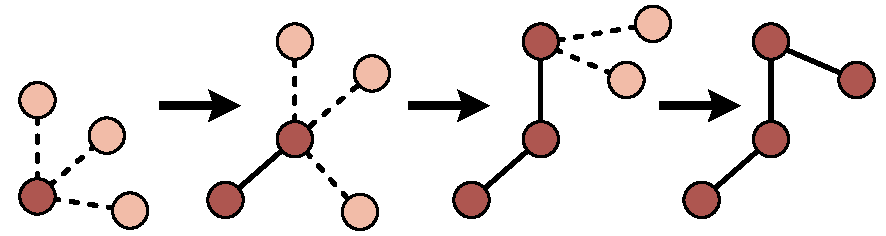
\includegraphics[width=0.9\textwidth]{figures/images/cbmc}
    \caption{Illustration of a single configurational bias Monte Carlo move. A
    linear molecule is regrown step by step. At each step, the position for the
    next atom is picked at random, depending on the position of all the
    previous atoms.}
    \label{fig:cbmc}
\end{figure}

The main issues with configuration bias Monte Carlo is that it requires
knowledge of all the separated intra-molecular interaction terms to be able to
generate the position of the next atom while maintaining detailed balance; and
not only the global energy change as for simpler moves. It is also harder to use
it for even the simplest branched molecules.

Flexible nanoporous materials add another level of difficulty for efficient
Monte Carlo simulations. Some of them display collective behavior linked to
global deformations of the simulation cell, such as breathing in MIL-53 or some
cases of gate-opening. Here, the volume of the simulation cell changes as the
linkers rotate and move, thus needing Monte Carlo moves able to sample both the
collective rotation of linkers and the changes in the unit cell shape and
volume. It is possible to use molecular dynamics instead of Monte Carlo to
explore the response of the material to an external stress, as molecular
dynamics simulations are very efficient when sampling collective behaviors. But
when the stress is created by adsorbed molecules, we need to use grand canonical
Monte Carlo (see section~\ref{sec:gcmd}). Hybrid Monte Carlo is a technique that
can bridge the gap between traditional Monte Carlo and molecular dynamics,
bringing the ability to sample such collective motions to a Monte Carlo
simulation\cite{Rogge2019}.

In addition to being able to improve the sampling efficiency of Monte Carlo
simulations, Hybrid Monte Carlo can bring the power of non-physical moves in
simulations usually relying on molecular dynamics. For example, the study of
large bio-molecules --- the typical example is the simulation of protein folding
--- is often limited by the time scale at which the simulation can produce a new
conformation, decorrelated from the previous one\cite{Izaguirre2004}. Monte
Carlo can help to reduce this time by allowing jump from one conformation to
another, and incorporate domain specific knowledge (which part of the protein
can rotate, which parts will move together) to improve simulation efficiency.

Another area that can see improvements by incorporating non-physical moves is
the simulation of diluted aqueous environment, such as the salt and pH
environment around proteins. The pH of human blood is constant around 7.4,
meaning that both \ce{HO-} and \ce{H+} ions are only present at concentration
around \SI{e-7}{mol/L}. If we want to simulate a realistic pH environment, we
need to simulate more than 500 million water molecule for each \ce{HO-} or
\ce{H+} ion. In addition to that, because the surface of proteins can carry
non-neutral charges, the local ion concentration can depart from the measured,
global concentration in blood plasma or cell's cytoplasm. Grand Canonical and
semi-Grand Canonical Monte Carlo moves used together with Hybrid Monte Carlo can
bring realistic salt and pH condition to these simulations\cite{Ross2018}.

\subsection{Mixing molecular dynamics and Monte Carlo}

Hybrid Monte Carlo was first devised in 1987 by \citeauthor{Duane1987} for
calculations in lattice quantum chromodynamics \cite{Duane1987}. It was then
adapted to condensed matter molecular simulation by \citeauthor{Mehlig1992} in
1992\cite{Mehlig1992}. The central idea is to use a short molecular dynamics
simulation (around 10 steps) to generate a new conformation for the Markov
chain. Once the molecular dynamics simulation finished, the final step is
considered as a trial conformation, and accepted or rejected with the adapted
Metropolis criterion.

One global move in \emph{configuration space} consists in propagating the system
through \emph{phase space} for a fixed number of steps using some integration
scheme $\psi_{\delta t}$ of Hamilton's equations. $\psi_{\delta t}$ depends on
the integration time step $\delta t$ and the Hamiltonian of the system
$\mathcal{H}$; and maps the initial configuration $(\r, \v)$ in phase space to
the final one $(\r', \v')$:
\[\begin{array}{llcl}
    \psi_{\delta t} : & \mathbb{R}^{6N} & \longrightarrow & \mathbb{R}^{6N} \\
                      & (\r, \v)        & \longmapsto     & \psi_{\delta t}(\r, \v) \equiv (\r', \v')
\end{array}\]

Since the usual Monte Carlo scheme does not uses the atomic velocities, we need
to generate new velocities before starting the molecular dynamics simulation. We
choose to generate them according the the canonical ensemble distribution at
temperature $T$:
\[ \mathcal{P}_T(\v) \propto \exp\left(- \beta \sum_i \frac 12 m_i \v_i^2 \right)\]

Following the same notations as in chapter~\ref{sec:molsim}, because the time
integration is deterministic, the probability $\alpha(\r \to \r')$ to generate a
given conformation $\r'$ starting from $\r$ is the same as the probability to
generate a specific set of initial velocities $\mathcal{P}_T(\v)$:
\[ \alpha(\r \to \r')\ \d\r' = \mathcal{P}_T(\v) \ \d\v \]

If we use an acceptation probability that depends on the discretization error
$\delta \mathcal{H}$:
\begin{gather}
    \text{acc}((\r, \v) \to (\r', \v')) = \min\left(1, e^{-\beta \delta \mathcal{H}}\right), \\
    \delta \mathcal{H} = \mathcal{H}(\r', \v') - \mathcal{H}(\r, \v);
\end{gather}
we can show that the resulting Monte Carlo move respect the detailed balance
provided that the integration scheme $\psi_{\delta t}$ is \emph{time reversible}
and \emph{symplectic}.
\[\begin{array}{lcllll}
    \mathcal{P}(\r)\ \pi(\r \to \r') \ \d\r\d\v   &=& \mathcal{P}(\r)  & \mathcal{P}_T(\v)  & \text{acc}\kern-0.5ex\left((\r, \v) \to \psi_{\delta t}(\r, \v)\right)      & \d\r\d\v \\
    \text{\footnotesize \itshape see below}       &=& \mathcal{P}(\r') & \mathcal{P}_T(\v') & \text{acc}\kern-0.5ex\left(\psi_{\delta t}(\r, \v) \to (\r, \v)\right)      & \d\r\d\v \\
    \text{\footnotesize \itshape time reversible} &=& \mathcal{P}(\r') & \mathcal{P}_T(\v') & \text{acc}\kern-0.5ex\left((\r', \v') \to \psi_{-\delta t}(\r', \v')\right) & \d\r\d\v \\
    \text{\footnotesize \itshape symplectic}      &=& \mathcal{P}(\r') & \mathcal{P}_T(\v') & \text{acc}\kern-0.5ex\left((\r', \v') \to \psi_{-\delta t}(\r', \v')\right) & \d\r'\d\v' \\
                                                  &=& \mathcal{P}(\r') & \multicolumn{2}{l}{\pi(\r' \to \r) \ \d\r'\d\v'}
\label{eq:hmc-demonstration}
\end{array}\]
The first step in the above demonstration comes from the mathematical identity
\[e^{-\beta\mathcal{H}(\r, \v)} \min\kern-0.5ex\left(1, e^{-\beta \delta \mathcal{H}}\right) = e^{-\beta\mathcal{H}(\r', \v')} \min\kern-0.5ex\left(e^{\, \beta \delta \mathcal{H}}, 1\right). \]

It is worth noting that even though the molecular dynamics simulation evolves in
the micro-canonical $NVE$ ensemble, the overall HMC simulation is sampling the
canonical $NVT$ ensemble. This allow to use HMC simulations as a rigorous way to
sample the $NVT$ ensemble using molecular dynamics.

The acceptance rate of the hybrid moves is dictated by the value of
$\delta\mathcal{H}$. This value is the discretization error associated with the
timestep used by the molecular simulation, and depends only on $\delta t$ and
the number of steps used to propagate the system with molecular dynamics. These
are the parameters we can adjust to change the global acceptance rate.

\subsubsection{Constant pressure simulations}

There are two ways to use Hybrid Monte Carlo simulations to sample the
isobaric-isothermal $NPT$ ensemble. The first one is to use separate moves to
change the volume and the particles' positions --- the former using standard
Monte Carlo moves and the latter relying on hybrid moves. While doing so is
simpler from an implementation point of view, it can be less efficient when the
changes in volume are coupled to local deformations of the system.

Another possibility is to use the hybrid moves to sample both the volume changes
and the particles' displacements. The same construction used above can be used
to create an hybrid move that sample the $NPT$ ensemble. The molecular dynamics
integrator now maps the initial position in phase space including the volume $V$
$(V, \r, \v)$ to a new position in phase space $(V', \r', \v')$. If the
integrator is deterministic, the probability to generate a specific new state
from the initial one $\alpha((V, \r) \to (V', \r'))$ is still the same as the
probability to generate the initial  velocities $\mathcal{P}_T(\v)$. Provided
the integrator is time reversible and symplectic, the same demonstration as in
equation~\eqref{eq:hmc-demonstration} applies by adapting the acceptance
criterion to
\[\text{acc}((V, \r, \v) \to (V', \r', \v')) = \min\left(1, e^{-\beta \delta \mathcal{H} - \beta\ P \Delta V}\right)\]

If an extended Langrangian integrator such as the one proposed by
Andersen\cite{Andersen1980} is used, the momentum of the fictitious external
\emph{piston} should also be included in both the probability of creating a new
state $\alpha((V, \r) \to (V', \r'))$ and in the Hamiltonian part of the
acceptance criterion\cite{Faller2002, FernandezPendas2014}.

Again, we should note that the molecular dynamics simulation only samples the
is\-enthalpic-iso\-baric $NPH$ ensemble, and the Monte Carlo acceptance criterion
ensure sampling of the isobaric-isothermal $NPT$ ensemble. Actually, the
molecular dynamics does not even need to sample an accurate $NPH$ ensemble, only
to generate new states with different volume and following the above properties
of being deterministic, time-reversible and symplectic. The Metropolis
acceptance criterion ensures that the correct ensemble will be sampled.

\subsubsection{Osmotic simulations}

Once we are able to use hybrid simulations to sample the $NPT$ ensemble, moving
to the osmotic $N_\text{host}\,\mu\,PT$ ensemble is accomplished by adding
insertion/deletion moves to allow the number of adsorbed particles to vary. Very
recently, \citeauthor{Rogge2019}\cite{Rogge2019} used such hybrid Monte Carlo
simulations to study adsorption of noble gases, \ce{CO2} and \ce{CH4} in
MIL-53(Al) using the osmotic ensemble. They were able to reach very good
agreement with experimental measurements of adsorption isotherms and predict the
bi-stability and breathing of MIL-53(Al) upon adsorption.

Because the correctness of the sampled ensemble is validated by the Metropolis
criterion and the detailed balance, hybrid moves are not required to produce
statistically correct ensemble. This means that it should be possible to use an
adapted Grand Canonical Molecular Dynamics scheme to generate new trial
conformation to be accepted with the Metropolis criterion. To my knowledge, this
as not been attempted yet, but could improve insertion rate for osmotic
simulations in dense phases --- such as the simulation of intrusion in porous
solids. Traditional insertion/deletion moves suffer from a very low acceptance
rate in dense phases such as liquids, because molecules are already densly
packed and there is not enough space to add new molecules. Grand canonical
molecular dynamics can help by progressively scaling the \emph{presence} of the
new molecule up, allowing its surroundings to relax.

\subsubsection{Related algorithms and methods}

In the last decade, some improvements to the simple hybrid Monte Carlo method
presented here have been proposed. Shadow Hybrid Monte Carlo\cite{Izaguirre2004}
relies on the existence and computability of a \emph{shadow} Hamiltonian being
propagated exactly (without any propagation error) by $\psi_{\delta t}$ to
improve the acceptance rate of hybrid moves, and reconstruct \emph{a posteriori}
the probabilities of each generated conformation. Generalized Hybrid Monte
Carlo\cite{Akhmatskaya2009, Akhmatskaya2011} uses configurations in the phase
space instead of conformations in the Markov chain, keeping the velocities from
one Monte Carlo move to another. The different steps are still accepted or
rejected by a Metropolis criterion, and velocities are partially updated with
new random values at each step. The combination of these two approaches is
called Generalized Shadow Hybrid Monte Carlo, and implemented in the GROMACS
simulation software\cite{FernandezPendas2014}. Finally, tentative to lift
the symplectic requirement on the integrator are at the origin of Compressible
Generalized Hybrid Monte Carlo\cite{Fang2014}.

\subsection{Hybrid simulations of adsorption}

I used my implementation of hybrid Monte Carlo in Domino to study adsorption of
methane \ce{CH4} in MOF-5 at \SI{300}{K}. I used a simplified model of both
MOF-5 and \ce{CH4} as Domino did not support computing electrostatic
interactions at the time. \ce{CH4} molecules where approximated by a single
spherical Lennard-Jones sphere, using $\sigma = \SI{3.737}{\AA}$ and $\epsilon =
\SI{1.247}{kJ/mol}$. I used the Lennard-Jones and intra-molecular terms from
QuickFF\cite{Vanduyfhuys2015}, ignoring the atomic charges. While the resulting
model is not an accurate representation of MOF-5, it is still an interesting
test case for the use of hybrid Monte Carlo simulations in adsorption.

To obtain a full isotherm , I ran 8 simulations at different \ce{CH4} pressures.
Each simulation used two Monte Carlo moves: insertion/deletion of \ce{CH4}
taking the current pressure as the gas fugacity; and hybrid moves. The hybrid
moves used a Velocity-Verlet integrator with a timestep of \SI{1}{fs}, and a
Berendsen barostat setting the external pressure at the same value as the
\ce{CH4} fugacity and a time step of \SI{5}{ps}. I should point out that I used
the Berendsen barostat even if it is not symplectic nor time reversible, as it
was the only barostat implemented in Domino. Again, while the resulting
simulation might not sample the adequate ensemble, it is still and interesting
check. Each simulation was propagated for a million of Monte Carlo moves, using
the first 250 000 moves as the equilibration period. The resulting isotherms is
shown in figure~\ref{fig:hmc-mof5} together with the changes in volume as the
pressure increases.

\begin{figure}[ht]
    \centering
    % GNUPLOT: LaTeX picture with Postscript
\begingroup
  \makeatletter
  \providecommand\color[2][]{%
    \GenericError{(gnuplot) \space\space\space\@spaces}{%
      Package color not loaded in conjunction with
      terminal option `colourtext'%
    }{See the gnuplot documentation for explanation.%
    }{Either use 'blacktext' in gnuplot or load the package
      color.sty in LaTeX.}%
    \renewcommand\color[2][]{}%
  }%
  \providecommand\includegraphics[2][]{%
    \GenericError{(gnuplot) \space\space\space\@spaces}{%
      Package graphicx or graphics not loaded%
    }{See the gnuplot documentation for explanation.%
    }{The gnuplot epslatex terminal needs graphicx.sty or graphics.sty.}%
    \renewcommand\includegraphics[2][]{}%
  }%
  \providecommand\rotatebox[2]{#2}%
  \@ifundefined{ifGPcolor}{%
    \newif\ifGPcolor
    \GPcolortrue
  }{}%
  \@ifundefined{ifGPblacktext}{%
    \newif\ifGPblacktext
    \GPblacktextfalse
  }{}%
  % define a \g@addto@macro without @ in the name:
  \let\gplgaddtomacro\g@addto@macro
  % define empty templates for all commands taking text:
  \gdef\gplbacktext{}%
  \gdef\gplfronttext{}%
  \makeatother
  \ifGPblacktext
    % no textcolor at all
    \def\colorrgb#1{}%
    \def\colorgray#1{}%
  \else
    % gray or color?
    \ifGPcolor
      \def\colorrgb#1{\color[rgb]{#1}}%
      \def\colorgray#1{\color[gray]{#1}}%
      \expandafter\def\csname LTw\endcsname{\color{white}}%
      \expandafter\def\csname LTb\endcsname{\color{black}}%
      \expandafter\def\csname LTa\endcsname{\color{black}}%
      \expandafter\def\csname LT0\endcsname{\color[rgb]{1,0,0}}%
      \expandafter\def\csname LT1\endcsname{\color[rgb]{0,1,0}}%
      \expandafter\def\csname LT2\endcsname{\color[rgb]{0,0,1}}%
      \expandafter\def\csname LT3\endcsname{\color[rgb]{1,0,1}}%
      \expandafter\def\csname LT4\endcsname{\color[rgb]{0,1,1}}%
      \expandafter\def\csname LT5\endcsname{\color[rgb]{1,1,0}}%
      \expandafter\def\csname LT6\endcsname{\color[rgb]{0,0,0}}%
      \expandafter\def\csname LT7\endcsname{\color[rgb]{1,0.3,0}}%
      \expandafter\def\csname LT8\endcsname{\color[rgb]{0.5,0.5,0.5}}%
    \else
      % gray
      \def\colorrgb#1{\color{black}}%
      \def\colorgray#1{\color[gray]{#1}}%
      \expandafter\def\csname LTw\endcsname{\color{white}}%
      \expandafter\def\csname LTb\endcsname{\color{black}}%
      \expandafter\def\csname LTa\endcsname{\color{black}}%
      \expandafter\def\csname LT0\endcsname{\color{black}}%
      \expandafter\def\csname LT1\endcsname{\color{black}}%
      \expandafter\def\csname LT2\endcsname{\color{black}}%
      \expandafter\def\csname LT3\endcsname{\color{black}}%
      \expandafter\def\csname LT4\endcsname{\color{black}}%
      \expandafter\def\csname LT5\endcsname{\color{black}}%
      \expandafter\def\csname LT6\endcsname{\color{black}}%
      \expandafter\def\csname LT7\endcsname{\color{black}}%
      \expandafter\def\csname LT8\endcsname{\color{black}}%
    \fi
  \fi
    \setlength{\unitlength}{0.0500bp}%
    \ifx\gptboxheight\undefined%
      \newlength{\gptboxheight}%
      \newlength{\gptboxwidth}%
      \newsavebox{\gptboxtext}%
    \fi%
    \setlength{\fboxrule}{0.5pt}%
    \setlength{\fboxsep}{1pt}%
\begin{picture}(7360.00,2820.00)%
    \gplgaddtomacro\gplbacktext{%
      \csname LTb\endcsname%%
      \put(543,595){\makebox(0,0)[r]{\strut{}$0$}}%
      \csname LTb\endcsname%%
      \put(543,886){\makebox(0,0)[r]{\strut{}$5$}}%
      \csname LTb\endcsname%%
      \put(543,1177){\makebox(0,0)[r]{\strut{}$10$}}%
      \csname LTb\endcsname%%
      \put(543,1468){\makebox(0,0)[r]{\strut{}$15$}}%
      \csname LTb\endcsname%%
      \put(543,1760){\makebox(0,0)[r]{\strut{}$20$}}%
      \csname LTb\endcsname%%
      \put(543,2051){\makebox(0,0)[r]{\strut{}$25$}}%
      \csname LTb\endcsname%%
      \put(543,2342){\makebox(0,0)[r]{\strut{}$30$}}%
      \csname LTb\endcsname%%
      \put(543,2633){\makebox(0,0)[r]{\strut{}$35$}}%
      \csname LTb\endcsname%%
      \put(645,409){\makebox(0,0){\strut{}$0$}}%
      \csname LTb\endcsname%%
      \put(1100,409){\makebox(0,0){\strut{}$10$}}%
      \csname LTb\endcsname%%
      \put(1554,409){\makebox(0,0){\strut{}$20$}}%
      \csname LTb\endcsname%%
      \put(2009,409){\makebox(0,0){\strut{}$30$}}%
      \csname LTb\endcsname%%
      \put(2464,409){\makebox(0,0){\strut{}$40$}}%
      \csname LTb\endcsname%%
      \put(2918,409){\makebox(0,0){\strut{}$50$}}%
      \csname LTb\endcsname%%
      \put(3373,409){\makebox(0,0){\strut{}$60$}}%
    }%
    \gplgaddtomacro\gplfronttext{%
      \csname LTb\endcsname%%
      \put(153,1614){\rotatebox{-270}{\makebox(0,0){\strut{}intake (\% wt)}}}%
      \csname LTb\endcsname%%
      \put(2009,130){\makebox(0,0){\strut{}pressure (bar)}}%
    }%
    \gplgaddtomacro\gplbacktext{%
      \csname LTb\endcsname%%
      \put(4427,595){\makebox(0,0)[r]{\strut{}$16.8$}}%
      \csname LTb\endcsname%%
      \put(4427,1003){\makebox(0,0)[r]{\strut{}$17$}}%
      \csname LTb\endcsname%%
      \put(4427,1410){\makebox(0,0)[r]{\strut{}$17.2$}}%
      \csname LTb\endcsname%%
      \put(4427,1818){\makebox(0,0)[r]{\strut{}$17.4$}}%
      \csname LTb\endcsname%%
      \put(4427,2225){\makebox(0,0)[r]{\strut{}$17.6$}}%
      \csname LTb\endcsname%%
      \put(4427,2633){\makebox(0,0)[r]{\strut{}$17.8$}}%
      \csname LTb\endcsname%%
      \put(4529,409){\makebox(0,0){\strut{}$0$}}%
      \csname LTb\endcsname%%
      \put(4950,409){\makebox(0,0){\strut{}$10$}}%
      \csname LTb\endcsname%%
      \put(5370,409){\makebox(0,0){\strut{}$20$}}%
      \csname LTb\endcsname%%
      \put(5791,409){\makebox(0,0){\strut{}$30$}}%
      \csname LTb\endcsname%%
      \put(6212,409){\makebox(0,0){\strut{}$40$}}%
      \csname LTb\endcsname%%
      \put(6632,409){\makebox(0,0){\strut{}$50$}}%
      \csname LTb\endcsname%%
      \put(7053,409){\makebox(0,0){\strut{}$60$}}%
    }%
    \gplgaddtomacro\gplfronttext{%
      \csname LTb\endcsname%%
      \put(3833,1614){\rotatebox{-270}{\makebox(0,0){\strut{}volume (\si{nm^3})}}}%
      \csname LTb\endcsname%%
      \put(5791,130){\makebox(0,0){\strut{}pressure (bar)}}%
    }%
    \gplbacktext
    \put(0,0){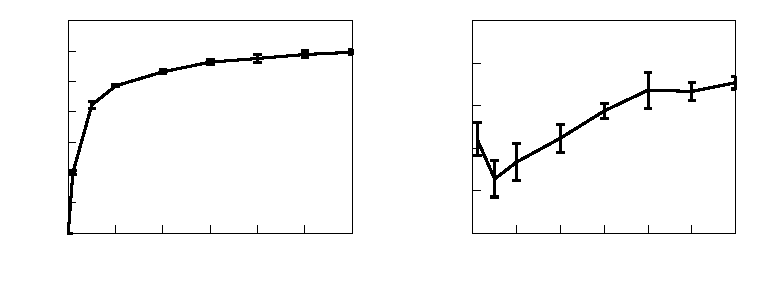
\includegraphics{hmc-mof5}}%
    \gplfronttext
  \end{picture}%
\endgroup

    \caption{Hybrid Grand Canonical Monte Carlo simulations results for the
    adsorption of methane in a simplified MOF-5 model. (left) adsorption
    isotherm at \SI{300}{K}, (right) volumes changes during adsorption.}
    \label{fig:hmc-mof5}
\end{figure}

The resulting isotherm is a simple type I isotherm, as expected for the
adsorption of methane in MOF-5. More interesting is the non-monotonous behavior
of the curve of volume deformations as a function of pressure. We first see a
small contraction of the unit cell at low loading, before the expected increase
at higher pressures. This contract--expand behavior is reminiscent of
sorption-induced deformation in other porous materials\cite{Balzer2013,
Mouhat2015}: the presence of few molecules inside the pores induces a
\emph{softening} and a contraction of the whole system. Another way to look at
this phenomenon is to envision the molecules inside the pore \emph{pulling} on
the pores wall.

It is remarkable to see that a simple model of the MOF is able to reproduce this
relatively complex behavior. In order to improve the model and predictive
possibilities of hybrid Monte Carlo simulations, I needed to implement a way to
compute electrostatics interactions. In the next section, I will discuss two
methods one can use to compute these interactions in the presence of periodic
boundary conditions.

% \newpage
\section{Computation of electrostatic energy in classical simulations}
\label{sec:electrostatic}

Classical force fields represent the energy of an atomic system as a sum of
multiple contributions, including dispersion and short-range repulsion,
intra-molecular interactions and electrostatic interactions. In the last case,
atoms are often identified to point charges, interacting through a Coulombic
potential. For two atoms $i$ and $j$ carrying charges $q_i$ and $q_j$, at a
distance $r$ from one another, this potential reads:
\[ V(r) = \frac{q_i q_j}{4 \pi \epsilon_0 r}.\]
In the remaining of this chapter, I will be using units such that $4 \pi
\epsilon_0 = 1$.

\subsection{The problem}

As presented in section~\ref{sec:pbc}, we are limited in the size of systems we
can simulate with classical simulation methods. To remove the size and surface
effects arising from the relatively small number of particles in a simulation,
most if not all classical simulations uses the trick of periodic boundary
conditions. This means that we are in effect simulating an infinite system,
extending in all three dimensions of space. All of the interaction potentials
that have an action at long distances goes down to zero as the distance between
atoms goes to infinity (else the overall energy would be infinite). It is thus
usual to use a cutoff radius $r_c$ when computing the energy of a system: any
interaction between atoms further apart than this radius is supposed negligible,
and set to zero. This allows to speed up the calculation of energies in the
simulations by ignoring many small contributions. The error $\epsilon$ arising
from the use of a cutoff radius can be quantified --- using $V(r)$ for the pair
potential:
\[\epsilon = \int_{r_c}^\infty r^2 V(r)\ \d r. \]
This error can be computed and used to correct after the fact the energy and
pressure computed from a simulation. This correction is called the
\emph{long-range} or \emph{tail} correction.

Unfortunely, the above integral only converges if $V(r)$ goes to zero faster
than $1/r^3$, which is not the case for the electrostatic potential. In the
following, I will be describing two methods one can use to compute the
electrostatic interaction accurately in classical molecular simulations: Ewald
summation and Wolf summation. I implemented both in the Domino project, and I
will give some software tricks I used to speed up the implementations.

\subsection{Ewald summation}

Ewald summation was proposed by Paul Peter Ewald in 1921\cite{Ewald1921}

\subsection{Wolf summation}

Papier originel de la méthode de Wolf\cite{Wolf1999}: on utilise le fait que le
potentiel effectif d'un multipole complexe est de l'ordre de $1/r^5$ pour
effectuer le calcul de l'énergie de Madelung via un simple somme de paires avec
un terme correctif. Ceci est équivalent à l'utilisation d'un potentiel
\emph{shifté}:
\[V_{SP}(r) = q_i q_j \left(\frac{1}{r} - \frac{1}{r_c} \right) \text{pour } r < r_c\]

Pour ne pas avoir besoin de rayons de coupure énormes, on utilse un potentiel amorti:
\[V_{DSP}(r) = \frac{q_i q_j \ \erfc(\alpha r)}{r} - \lim_{r \to r_c} \frac{q_i q_j \ \erfc(\alpha r)}{r}\]
\[\vec f_{ij}^{\ DSP} = q_i q_j \left[\frac{\erfc(\alpha r)}{r^2} + \frac{2\alpha}{\sqrt{\pi}} \frac{\exp(-\alpha^2 r^2)}{r}\right] \frac{\vec r}{r}
- q_i q_j \left[\frac{\erfc(\alpha R_c)}{R_c^2} + \frac{2\alpha}{\sqrt{\pi}} \frac{\exp(-\alpha^2 R_c^2)}{R_c}\right] \frac{\vec r}{r}\]


Les formules ci-dessus ont l'inconvénient de ne pas être $\mathcal{C}^1$ en $r_c$. Ce
papier\cite{Fennell2006} propose de partir de la force, et d'intégrer pour obtenir le potentiel
correspondant. On obtient:

\[\vec f_{ij}^{\ DSF} = q_i q_j \left[\frac{\erfc(\alpha r)}{r^2} + \frac{2\alpha}{\sqrt{\pi}} \frac{\exp(-\alpha^2 r^2)}{r}\right] \frac{\vec r}{r}
- q_i q_j \left[\frac{\erfc(\alpha R_c)}{R_c^2} + \frac{2\alpha}{\sqrt{\pi}} \frac{\exp(-\alpha^2 R_c^2)}{R_c}\right] \frac{\vec r}{r}\]

\[V_{DSF}(r) = q_i q_j \left[\frac{\erfc(\alpha r)}{r} - \frac{\erfc(\alpha r_c)}{r_c}
+ \left(\frac{\erfc(\alpha r_c)}{r_c^2} + \frac{2\alpha}{\sqrt{\pi}} \frac{\exp(-\alpha^2 r_c^2)}{r_c}\right) (r - r_c)\right]\]


\TODO \cite{Fukuda2013}

\subsection{Comparing Ewald and Wolf}

\OnlyInSubfile{\printbibliography}

\end{document}
